51. На рисунке изображена буква {\bf Т} ширины 7, высоты 6, а толщина ножки и шляпки у неё 3 клетки. Сколько клеток содержит аналогичная буква {\bf Т} ширины 70, высоты 60 и толщиной ножки и шляпки 6 клеток?
\begin{center}
\begin{figure}[ht!]
\center{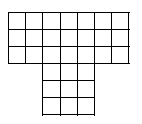
\includegraphics[scale=0.35]{9.png}}
\end{figure}
\end{center}
\newpage
\noindent52. На рисунке изображена буква {\bf Т} ширины 7, высоты 6, а толщина ножки и шляпки у неё 3 клетки. Сколько клеток содержит аналогичная буква {\bf Т} ширины 60, высоты 70 и толщиной ножки и шляпки 8 клеток?
\begin{center}
\begin{figure}[ht!]
\center{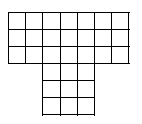
\includegraphics[scale=0.35]{9.png}}
\end{figure}
\end{center}
